\section{Implementation}

This section starts by describing some important algorithms and implementation details of Atmosphere.

\subsection{Data structures and algorithms}

This subsection describes data structures and algorithms used in both JavaScript and Cocoa implementations. Later subections discuss platform specific implementation details.

Both implementations provide object-oriented system of code organization. Components of Atmosphere are represented using classes as pictured in Figure \ref{fig:1}.

\begin{figure}[ht!]
\centering
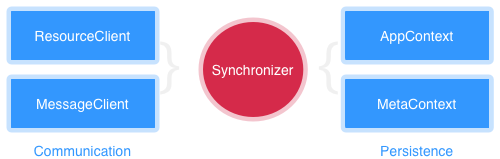
\includegraphics[width=350pt]{GeneralImplementation.png}
\caption{Classes used in implementation of Atmosphere \label{fig:1}}
\end{figure}

\subsubsection{Communication}

The communication layer consists of two classes: The resource client and the message client.

\textbf{Resource client} is used to download data over HTTP protocol conforming to REST style. In order to make a HTTP request, we need a URL for the resource. The process of converting a model and action pair to URL string is called routing. It is done by specifying an application specific routing table similiar to one pictured in Figure \ref{fig:Routing}.

\begin{figure}[htbp]
  \centering
    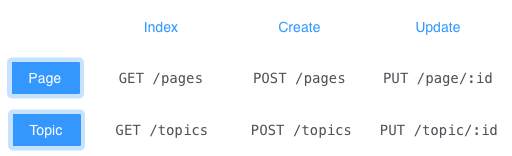
\includegraphics[width=300pt]{Routing.png}
  \caption{Example routing table for resource client}
  \label{fig:Routing}
\end{figure}

Once the correct URL is looked up in the table, the resource client prepends the base URL for the REST source, replaces occurences of ID string with ID of record being saved, processes extra request-specific options and sends the request.

Resource client is also responsible for extracting data contained in the response returned from HTTP call. In the current implementation, only the JSON format is supported. Since the response could store data in many different ways (see Listing \ref{json}), Atmosphere allows setting custom function (or block in Objective-C) for retrieving these data from the JSON response.

\begin{lstlisting}[caption=Different formats of response JSON data,label=json]
// Simple JSON response
[{name: "Edukit"}, {name: "Atmosphere"}]
// More complicated JSON response
{"projects": [{"project": {name: "Edukit"}}, {"project": {name: "Atmosphere"}}]}
\end{lstlisting}


\subsection{JavaScript implementation}

At the time of writing, JavaScript implementation of Atmosphere is built on top of the Spine \citep{spinejs} library which is a lightweight framework for building JavaScript web applications.

The library doesn’t completely rely on Spine, instead it only utilizes its model layer. Furthermore, all the code that requires Spine is contained in one small file, which can be easily rewritten for other client side frameworks and their own model layers.

The implementation is written in CoffeeScript \citep{coffeescript}, which is a language that improves syntax of JavaScript by introducing many syntactic shortcuts such as semantic whitespace (inspired by Python) or accessing instance variables with the '@' sign. (inspired by Ruby).



The classes in persistence and communication layers implement the basic roles of Atmosphere, while the Synchronizer class is the entry point for working with Atmosphere.

The Spine integration contains shortcuts for calling Atmosphere methods directly from Spine models using the API users are already developers are already familiar with.




\subsection{Cocoa implementation}

The Cocoa implementation is packaged as Xcode framework. It is written in Objective-C and can be compiled for both desktop (Mac) and mobile (iPhone and iPad) platforms.

From the high level perspective, the Cocoa implementation is 